\chapter{Solving the Shortest Path Problem}
\todo[inline]{do I need to show pseudocode for all algos?}
\label{chap:solvingspp}

Over the years,
various algorithms have been developed 
to address the problem of finding the shortest path in different situations.
In this chapter,
notations and definitions for the shortest path problem is stated first, 
the theory for solving the shortest path problem is described next,
algorithms that are applicable for road networks are then summarised,
including the discussion of their advantages and drawbacks.

\todo[inline]{Big O analysis for all algorithms}
\todo[inline]{Need to talk about results, what should the reader pay attention to? What should they conclude?}
\todo[inline]{assume a path always exist between an OD pair}

\section{Notations and Definitions}
The Shortest Path Problem (SPP) is the problem of finding the shortest path from a given origin  to some destination.
There are two types of SPP hat are going to
be analysed in this chapter:
a single-source and a point to point SPP.  
The Frank-Wolfe algorithm in the TA involves
solving the single-source SPP by finding of shortest path going from one origin to every other destinations the network.
The Path Equilibration method in the TA
Solving the point to point SPP solves from one origin to a specific destination and is used in the Path Equilibration method. 

When solving SPP for a normal road network,
different measurements such as distance and travel exist for the road length.
But in traffic assignment,
the road length is measured in a monotonic non-decreasing travel time function,
\todo{monotonic non-decreasing - correct?}
which encapsulates information such as traffic flow, road capacity and travel speed.
This travel time function is always non-negative so taking advantage of this helps the selection of algorithms that uses this property.
\todo{show equation?}

Using notations from \citet{Cormen} and \citet{Klunder} and in the context
of transportation networks,
we denote $ G = ( V, E ) $ for a weighted, directed graph,
where $ V $ denotes the set of nodes (origins, destinations, and intersections)
and $ E $ the set of edges (roads);
we say $ E $ is a subset of the set $ \{ (u, v)\, | \, u, v \in V \} $ of all ordered pairs of nodes.
We denote the weight function $ c : E \rightarrow \mathbb{R} $ which assigns a cost (travel time) to any arc $ (u,v) \in E $.
We write the costs of arc $(u, v)$ as: $ c((u, v)) = c_{uv} $.

The path $P$ inside a transportation network has to be a directed simple path, 
which is a sequence of nodes and arcs $ (u_1, (u_1, u_2), u_2, \ldots , (u_{k-1}, u_k), u_k ) $
such that $ (u_i, u_{i+1}) \in E$ for $i = 1,\ldots,k-1$ and $u_i \neq u_j$ for all $ 1 \leq i < j \leq k$.
Note $u_1$ is the origin and $u_k$ is the destination of the path $P$, $u_1$ and $u_k$ together is called an O-D pair for this path.
For simplicity, we denote $s$ to be the source (origin) and $t$ to be the target (destination) for any path $P$.
%Finally we denote cost of the whole path $C(P) := \sum_{(u,v)\in P} c_{vw}$.

In a transportation network,
the origins and destinations are often called centroids or zones.
They are traffic analysis zones for generating trip demands and supplies
and hold information such as household income and employment information,
these information helps the understanding of trips that are produced and attracted within the zone.
The zones are conceptual nodes in the network and are untravellable,
which means a path between two zone nodes must not contain another zone node.
\todo[inline]{Maybe a picture of the network explain what the zones are.}

Through out the report,
run-time analysis (big O and other notations) is used to demonstrate the estimation of algorithms running time regarding their input size. 
\todo[inline]{How do I nicely say `let the reader refer to other resources?'
or do I desribe what big O notation is?}

\section{Generic Shortest Path Algorithm (GSP)}
A family of algorithms exist for solving SPP with directed non-negative length arcs,
in this section we describe the generic case for these
algorithms.

This family of algorithms aim at finding a 
vector ($d_1, d_2,\dots d_v$) of distance labels and its corresponding shortest path \citep{Klunder}.
Each $d_v$ keeps the least distance of any path going from $s$ to $v$, $d_v = \infty$ if no paths has been found.
A shortest path is optimal when it satisfies the following conditions:
\begin{align}
    d_v \leq d_u + c_{uv}, \quad \forall(u,v) \in E, \label{eq:Bellman1}\\
    d_v  =   d_u + c_{uv}, \quad \forall(u,v) \in P.
\end{align}
\todo[noline]{what is $P$?}
The inequalities~(\ref{eq:Bellman1}) is called Bellman's condition \citep{Bellman}.
In other words,
we wish to find a label vector $d$ which satisfies Bellman's condition for all of the vertices in the graph.
To maintain the label vector, the algorithm uses a queue $\mathcal{Q}$ to store the label distances.

In the label vector,
a node is said to be unvisited when $d_u = \infty$,
scanned when $d_u \neq \infty$ and is still in the queue,
and labelled when the node has been retrieved from the queue and its distance label cannot be updated further.
If a node is labelled then its distance value is guaranteed to represent the minimal distance from $s$ to $t$, Bellman's condition must have been satisfied.

In the generic shortest path algorithm,
we start by putting the origin node in the queue,
and then iteratively find the arc that violates the Bellman's condition (i.e., $d_v > d_u + c_{uv}$),
distance labels are set to a value which satisfies condition (\ref{eq:Bellman1}) to the corresponding node of that arc.
Shortest path going from $s$ to all other nodes in $V$ is found when (\ref{eq:Bellman1}) is satisfied for all arcs in $E$.
It may not be obvious but negative costs are permitted in the GSP but not negative cost cycles.

We use $p_u$ to denote the predecessor of node $u$.
The shortest path can be constructed by following the predecessor of the destination node $t$ back to the origin node $s$. $p_s$ is often set to $-1$ to indicate it does not have a predecessor.

\todo[inline]{diagram showing $u, v, c_{vw}$ etc.}

Algorithm~\ref{algo:gsp} \citep{Klunder} describes the generic shortest path algorithm mentioned above,
with an extra constraint required when solving a TA problem: travelling through zone nodes are not permitted.
In essence, this algorithm repeatedly selects node $u\in\mathcal{Q}$ and checks the violation of Bellman's condition for all emanating arcs of node $u$.
\begin{algorithm}
    \caption{The Generic Shortest Path Algorithm}
    \label{algo:gsp}
    \begin{algorithmic}[1]
        \Procedure{GenericShortestPath}{$s$}
        \State $\mathcal{Q} \gets \mathcal{Q} \cup \{s\}$ \Comment{initialise queue with source node}
        \State $p_s \gets -1$ \Comment{origin has no predecessor}
        \State $d_s \gets 0$
        \ForAll {$ u \in V : u \neq s $} \Comment{all nodes are unvisited except the source}
        \State $d_u \gets \infty$
    \EndFor

    \While{ $\mathcal{Q} \neq \emptyset$ }
    \State $ u \gets \text{next}(\mathcal{Q}) $ \Comment{select next node}
    \State $ \mathcal{Q} \gets \mathcal{Q} \setminus \{u\} $
    \If{ $u \neq \text{zone} $}
    \ForAll {$v : (u, v) \in E$} \Comment{check Bellman's condition for all successors of $u$}
    \If {$d_u + c_{vw} < d_v$}
    \State $d_v \gets d_u + c_{vw}$
    \State $p_v \gets u$
    \If {$v \notin \mathcal{Q}$} 
    \State $\mathcal{Q} \gets \mathcal{Q} \cup \{v\}$ \Comment{add node $v$ to queue if unvisited}
\EndIf
                    \EndIf
                \EndFor
            \EndIf
        \EndWhile
    \EndProcedure
\end{algorithmic}
\end{algorithm}

Algorithm~\ref{algo:gsp} is generic because of two reasons:
the rule for selecting the next node $u$ (the next function in line 8) and
the implementation for the queue $\mathcal{Q}$ is unspecified.
Different algorithms use different rules and implementations to give 
either the one-source or the point-to-point shortest path algorithm \citep{mplomer}.
The next two sections describes these rules and implementations.

\section{Label Correcting Algorithm}
\todo[inline]{pseudo code}
\label{section:labelcorrectingalgorithm}
The GSP is addressed as a label correcting algorithm when the queue is a first in first out (FIFO) queue.
\todo{Check if its FIFO or double ended queue}
Given the arc costs can be negative in the GSP,
and in order to satisfy the Bellman's conditions for all arcs,
the algorithm has to scan all arcs $|V|-1$ times,
giving a run time of $O(|V||E|)$.

In this algorithm,
the distance labels do not get permanently labelled when the next node in the queue is retrieved,
another node may `correct' this node's distance label again,
thus the name label correcting algorithm.
This algorithm is also called the Bellman–Ford–Moore algorithm credited to \citet{Bellman, Ford} and \citet{Moore}.

\section{Label Setting Algorithm}
\label{section:labelsettingalgorithm}
The classical algorithm for solving the single-source shortest path problem is the label setting algorithm published by \citet{Dijkstra}.
The algorithm is addressed as label setting because when the next node $u$ is retrieved from the queue,
it gets permanently labelled;
the shortest path going to this node is solved and 
the distance label represents the shortest length.
In order to achieve label setting, 
the queue $\mathcal{Q}$ is modified to always have the minimum distance label in front of the queue,
hence the algorithm iterates through every node in the graph exactly once,
labelling the next node $u$ in the order of non-decreasing distance labels.

The advantage of this algorithm over the label correcting algorithm is
that all nodes in the graph are only visited once;
the shortest path tree grows radially outward from the source node.
It is clear that when the next node in the queue is the destination node,
the algorithm can be stopped for the point to point SPP case,
which is desirable for the Path Equilibration method.

\subsection{Priority Queue}
The run time performance of the Dijkstra's algorithm depends heavily on the implementation of the queue for storing the scanned nodes,
\citet{Cormen} suggest the use of a min-priority queue,
which is a collection of data structures that always serve elements with higher priorities, in our case they are the nodes with shorter distance labels.

Algorithm~\ref{algo:p2pdijkstra} shows the use of the min-priority queue in Dijkstra's algorithm.
The min-priority queue has 3 main operations: Insert, Extract-Min and Decrease-Key.
The Insert operation (line $2$ and $17$ in Algorithm~\ref{algo:p2pdijkstra}) is used for adding new nodes to the queue, the Extract-Min operation (line 8) is used for getting the element with the minimum distance label and the Decrease-Key is used for updating the distance if the node is already in the queue.

\begin{algorithm}[H]
    \caption{Point to Point Dijkstra's Algorithm}
    \label{algo:p2pdijkstra}
    \begin{algorithmic}[1]
        \Procedure{Dijkstra}{$s, t$}
        \State $\text{Insert}(\mathcal{Q}\text{ , u})$ \Comment{initialise priority queue with source node}
        \State $p_s \gets -1$ \Comment{origin has no predecessor}
        \State $d_s \gets 0$
        \ForAll {$ u \in V : u \neq s $} \Comment{all nodes are unvisited except the source}
        \State $d_u \gets \infty$
    \EndFor

    \While{ $\mathcal{Q} \neq \emptyset$ }
    \State $ u \gets \text{Extract-Min}(\mathcal{Q}) $ \Comment{select next node with minimum value}
    \If{ u = t}
    \State $\text{Terminate Procedure}$ \Comment{finish if next node is the destination}
\EndIf
\If{ $u \neq \text{zone} $}
\ForAll {$v : (u, v) \in E$} \Comment{check Bellman's condition for all successors of $u$}
\If {$d_u + c_{vw} < d_v$}
\State $d_v \gets d_u + c_{vw}$
\State $p_v \gets u$
\If {$v \notin \mathcal{Q}$} 
\State $\text{Insert}(\mathcal{Q}, v)$ \Comment{add node $v$ to queue if unvisited}
\Else
\State $\text{Decrease-Key}(\mathcal{Q}, v)$ \Comment{else update value of $v$ in queue}
    \EndIf
\EndIf
                \EndFor
            \EndIf
        \EndWhile
    \EndProcedure
\end{algorithmic}
\end{algorithm}

According to \citet{Cormen},
min-priority queue can implemented via an array or different kinds of min-heap data structure.

In the array implementation,
the distance labels are stored in an array where the $n^{\text{th}}$ position gives the distance value for node $n$.
Each Insert and Decrease-Key operation in this implementation takes $O(1)$ time, and each Extract-Min takes $O(V)$ time (searching through the entire array), giving a overall time of $O(V^2 + E)$.

A min-heap is a tree-based data structure which satisfies the min-heap property:
the value of each node is smaller or equal to the value of its child nodes.
\citet{Cormen} shows that if the graph is sufficiently sparse (in particular $E = o(V^2/\log(V))$, the Dijkstra's algorithm can be improved with a binary min-heap. In this implementation, the binary tree takes $O(V)$ time, Extract-Min takes $O(\log(V))$ time for $|V|$ operations and Decrease-Key takes $O(\log(V))$ time for each $|E|$. The total running time is therefore $O((V+E)\log(V))$, which improves the array implementation.

The running time can be improved further using a Fibonacci heap
developed by \citet{Fredman}.
Where historically, the development of Fibonacci heaps was motivated by the observation that Dijkstra's algorithm typically makes many more Decrease-Key calls than Extract-Min calls.
In Fibonacci heap, each of the $|V|$ Extract-Min operations take $O(\log(V))$ amortized time,
and each of the $|E|$ Decrease-Key operations take only $O(1)$ amortized time,
which gives a total running time of $O(V\log(V)+E)$.

\section{Bidirectional Label Setting Algorithm} \label{section:bidirectional}
The Dijkstra's algorithm can be imagined to be searching radially outward like a circle with the origin in the centre and destination on the boundary.
Likewise, Dijkstra's algorithm can be used on the reverse graph (all arcs reversed in the graph) from the destination node.
Thus Dijkstra's algorithm can be run on the origin and destination simultaneously at the same time.
The motivation for doing this is because the number of scanned nodes can be reduced when searching bidirectionally:
two smaller circles growing outward radially in stead of a larger one.
\todo{illustrate this}
It is common to conclude that the shortest path is found when the two searches meet somewhere in the centre,
but this is not actually the case as there may exist another arc connecting the two frontiers of the searches that has a shorter path.
The correct termination criteria was first designed and implementation by \citet{Pohl} based on researches presented by \citet{Dantzig, Nicholson} and \citet{Dreyfus}.
\citet{Klunder} summarises the procedure and algorithm (Algorithm~\ref{algo:bidirectional}) for the termination criteria presented by \citet{Pohl}.

In Algorithm~\ref{algo:bidirectional},
two independent Dijkstra's algorithms are alternatively run on the forward  and reverse graph (forward and backward algorithm),
the algorithms terminate when a node is permanently labelled in both directions.   
Once the algorithms have terminated,
the correct shortest path is found by looking for a arc connecting the frontiers of the two searches that may yield a shorter path.
This extra condition increases the run time significantly because 
we have to search for all arcs that connect all labelled nodes in the forward search to all labelled nodes in the backward search.
\todo{Show theorem and proof?}

Note in Algorithm~\ref{algo:bidirectional},
$\mathcal{R}^s$ is the subset of nodes that are permanently labelled from $s$ with labels $d_v^s$ in the forward search, and 
$\mathcal{R}^t$ is the subset of nodes that are permanently labelled from $s$ with labels $d_v^t$ in the backward search.

\begin{algorithm}[H]
    \caption{Bidirectional Label Setting Algorithm }
    \label{algo:bidirectional}
    \begin{algorithmic}[1]
        \Procedure{Bidirectional}{$s, t$}
        \State Execute one iteration of the forward algorithm.
        If the next node $u$ is labelled permanently by the 
        backward algorithm $(u\in\mathcal{R}^t)$, go to step 3.
        Else, go to step 2.
        \State Execute one iteration of the backward algorithm.
        If the next node $u$ is labelled permanently by the
        forward algorithm $(u\in\mathcal{R}^s)$, go to step 3.
        Else, goto step 1.
        \State Find $\min\{\min\{d_v^s + c_{vw} + d_w^t | v \in \mathcal{R}^s, w \in \mathcal{R}^t, (v, w) \in E\}, d_u^s + d_u^t\}$, which gives the correct shortest path between $s$ and $t$.
    \EndProcedure
\end{algorithmic}
\end{algorithm}

In recent years,
\citet{Goldberg05} improved the bidirectional search using a better termination condition.
The termination condition and its method is described as follows.
During the forward and backward search,
we maintain the length of the shortest path seen so far, $\mu$, and its corresponding path. Initially, $\mu = \infty$.
When an arc $(v,w)$ is scanned by the forward search and $w$ has already been scanned in the reverse search (or vice versa),
we know the shortest $s-v$ and $w-t$ path have lengths $d_v^s$ and $d_w^t$ respectively.
If $\mu > d_v^s + c_{vw} + d_w^t$ then this path is shorter than the one detected before, 
so we update $u$ and its path accordingly.
The algorithm terminates when the search in one direction selects a node already scanned in the other direction.

\citet{GoldbergEPP} showed and proved a stronger termination condition on top of his previous one.
The searches can be stopped if the sum of the top priority queue values is greater than $\mu$:
\[
    \text{top}_f + \text{top}_r \geq \mu
\]
where $\text{top}_f$ and $\text{top}_r$ are the top priority queue values in the forward and reverse search, they the next minimum distance label that have not been labelled.
\todo{Show theorem and proof as well?}

\section{A* Search}
\todo[inline]{I have been using the word ``heuristic'' everywhere, is ``potential'' function more appropriate or are they interchangeable?}
%\todo[inline]{Do I need to describe SPP in LP sense? like solving the dual, etc.? (which may make the bidirectional A* search section more understandable, where the dual version of the SPP is used for the theory, o)}
Up until now,
the Dijkstra's algorithm does not take into account the location of the destination,
the shortest path tree is grown out radially until the destination is labelled.
In a traditional graph where actual distances are used for the distance labels,
a heuristic can be used to direct the shortest path tree to grow toward the destination (an ellipsoid in stead of a circle).
\todo{show figure}
If the heuristic estimate is the distance from each node to the destination,
and the estimate is smaller than or equal to the actual distance going to that destination,
then a shortest path can be found. This is called A* search or goad directed search, first described by \citet{Astar}.

Formally we define the following: Let $h_v$ be a heuristic estimate from node $v$ to $t$,
and apply Bellman's condition such that an optimal solution exist, that is 
\begin{align}
    &h_v \leq h_u + c_{uv}, \quad \forall(u,v) \in E \\
    &h(t) = 0,
\end{align}
where $t$ is the destination node.
This means the heuristic function $h$ must be admissible and consistent (monotonic):
it never overestimates the actual path length and the estimated cost of a node reaching its destination node is no greater than the estimated cost of its predecessors.
Note a consistent heuristic is also admissible but not the oppossite.
\citet{Astar} proves if the heuristic function (such as using geographical coordinates and Euclidean distance) is admissible and consistent,
then A* is guaranteed to find the correct shortest path with a better time performance by scanning less nodes and arcs.

In the Path Equilibration method,
geographical coordinates and Euclidean distances can not be used for the heuristic estimate because a travel time function is used for the length of the arcs.
Instead, zero-flow travel time from every node to the destination can be for the heuristic.
Zero-flow travel time is admissible and consistent and can be shown by
analysing the travel times function (Figure~\ref{fig:flowfunction}).
The travel times function is a monotonic non-decreasing function with the lowest value being the zero-flow travel times.
This means using zero-flow travel times as the heuristic estimate
is assured to be admissible
as no travel time can be lower than the zero flow travel at any time.
The heuristic function is consistent because the travel time from a node to the destination must be no longer than all its predecessors.

\begin{figure}[H]
    \centering
    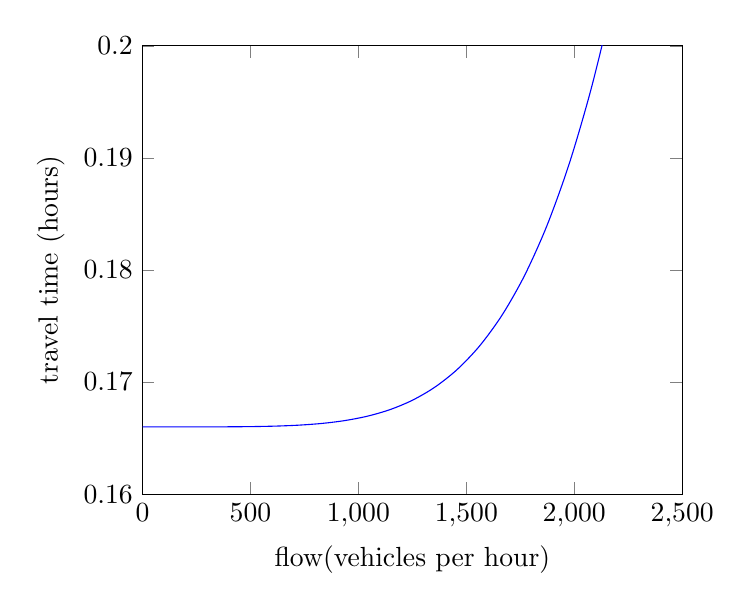
\begin{tikzpicture}
        \begin{axis}
            [
                domain=0:2500,
                black, no markers, smooth,
            %xtick=\empty, ytick=\empty,
                xlabel=flow(vehicles per hour), ylabel=travel time (hours),
                xmin=0,xmax=2500,
                ymin=0.16,ymax=0.2,
                yticklabel style={/pgf/number format/fixed, /pgf/number format/precision=3}
            ]
            \addplot {0.166*(1+0.15*(x/2000)^5)}; 
        \end{axis}
    \end{tikzpicture}
    \caption{Travel time function.}
    \label{fig:flowfunction}
\end{figure}
\todo{comment and correct graph}

\todo[inline]{mention the LP programming formulation, which may aid the explaintion of Bidirectional A*. See last paragraph in \url{http://en.wikipedia.org/wiki/Shortest_path_problem}}

\begin{comment}
\begin{algorithm}
Modifying Step 1 of the GSP for A* search:
    \caption{A* Search Algorithm}
    \begin{algorithmic}[1]
        \Procedure{AStar}{$s, t$}
        \State $\mathcal{Q} \gets \{s\}$ \Comment{Add node $s$ with $d_s = h_s$}
        \State $p_s \gets -1$
        \State $d_s \gets 0$
        \ForAll {$ u \in \mathcal{V} : u \neq s $} \Comment{All nodes unvisited except the source}
        \State $d_u \gets \infty$
    \EndFor

    \While{ $\mathcal{Q} \neq \emptyset$ }
    \State $ u \gets \text{top}(Q) $ \Comment{Remove $u$ such that $d_u + h_u = \displaystyle\min_{v \in \mathcal{Q}} \{ d_v + h_v \} $}
    \State $ \mathcal{Q} \gets \mathcal{Q} \char`\\ \{u\} $
    \If{ $u = t$ }
    \State \text{Terminate Procedure}
\EndIf
\If{ $u \neq \text{zone} $}
\ForAll {$v : (u, v) \in E$} \Comment{For all successors of $u$}
\If {$d_u + c_{vw} < d_v$}
\State $d_v \gets d_u + c_{vw}$
\State $p_v \gets u$
                        %\If {$v \notin \mathcal{Q}$} \Comment{Include node $v$ if unvisited}
\State $\mathcal{Q} \gets \mathcal{Q} \cup \{v\}$ \Comment{Add node $v$ with $d_v = d_u + c_{vw} + h_v$}
                        %\EndIf
                    \EndIf
                \EndFor
            \EndIf
        \EndWhile
    \EndProcedure
\end{algorithmic}
\todo[inline]{where are my $h$? heuristic?}
\end{algorithm}
\end{comment}

\section{Bidirectional A* Search}
Bidirectional search can also be applied to A* search,
where two ellipsoids are extended from the origin and destination respectively,
and construct the shortest path with the same strategy described in section~\ref{section:bidirectional}.
But this idea is wrong due to the independence use of the heuristic estimation in the two A* searches, and A* search does not label the nodes permanently in the order of their distance from the origin \citep{Klunder}.
In short, the heuristic estimations are no longer consistent.

The strategy for the correct use of heuristic estimates and termination criterion has first been published by \citet{Pohl}. The use of heuristic estimates is later improvement by \citet{Ikeda} and the termination criterion is improved by \citet{GoldbergEPP}.

The strategy is as follows. The heuristic estimates need to translated to consistent functions first. 
We denote $\pi_f(v)$ the estimate on distance from node $v$ to the destination $t$ in the forward search and $\pi_r(v)$ the estimate on distance from origin $s$ to node $v$ in the backward (reverse) search.
\todo{illustrate!}
In general two arbitrary feasible functions $\pi_f$ and $\pi_r$ are not consistent, but their average is both feasible and consistent \citep{Ikeda}:
\begin{align}
    p_f(v) = \frac{1}{2}(\pi_f(v)-\pi_r(v)) + \frac{\pi_r(t)}{2} \\
    p_r(v) = \frac{1}{2}(\pi_r(v)-\pi_f(v)) + \frac{\pi_f(s)}{2} 
\end{align}
where the two constants $\frac{\pi_r(t)}{2}$ and $\frac{\pi_f(s)}{2}$ are added by \citet{GoldbergEPP} to provide better estimates.
Note the modified consistent heuristic $p$ provides worse bounds than the original $\pi$ values.

Finally \citet{GoldbergEPP} shows and proves the stopping criterion:
\begin{align}
    \text{top}_f + \text{top}_r \geq \mu + p_r(t),
\end{align}
where is $\mu$ the best $s-t$ path seen fast, $\text{top}_f$ the length of the path from $s$ to the top node (minimum distance label) in the forward search priority queue and $\text{top}_r$ the length of the path from $t$ to the top node in the backward search priority queue.



\newpage
\todo[inline]{the following section is in draft stage}
\section{Preprocessing and More}
Preprocessing - trade memory to get faster time.
We can either do a fast preprocessing between iterations to make query in each iteration (so combined speed is still faster) 
or do a long preprocessing at the start and use the computed heuristic values
\begin{itemize}
    \item A* landmarks and triangle inequality (ALT)
    \item Reach-based routing 
    \item ALT + Reach
    \item Geometric Containers
    \item Arc Flags
\end{itemize}

If we have more data on the network we can use
algorithms that use hierarchies.
Consider roads with higher speed first: use a hierarchy of subgraphs.
\begin{itemize}
    \item Radius search.
    \item multi-level approach
    \item highway hierarchies
\end{itemize}

\todo[inline]{Above extract from: Speed-Up Techniques for Shortest-Path Computations by Dorothea Wagner, Thomas Willhalm, and Fast Shortest Path Algorithms for Large Road Networks by Faramroze Engineer }

We can also do Lifelong Planning A* (LPA*), use heuristic from previous each iteration, but the original paper says only a few percent arc change can boost run time, not idea if it is more than that. 

If the edge lengths are whole numbers then we can use multi-level bucket for the priority queue.


